\documentclass[a4paper,11pt]{article}
\usepackage[bottom=0.8in,top=0.8in, left=0.8in,right=0.8in]{geometry}

% non-numbered pages
\pagestyle{empty} 

%%%%%%%%%%% pdflatex %%%%%%%%%
\usepackage[T1]{fontenc}
\usepackage{newtxmath,newtxtext}
%%%%%%%%%%%%%%%%%%%%%%%%%%%%%%

%%%%%%%%%%% xelatex %%%%%%%%%%%%%%
% \usepackage{fontspec}
% \setmainfont{Times New Roman}
% \setmainfont{TeX Gyre Termes}
%%%%%%%%%%%%%%%%%%%%%%%%%%%%%%%%%%%

%A Few Useful Packages
\usepackage{parskip}
\usepackage{titlesec}	
\usepackage{multirow}
\usepackage{graphicx}
\usepackage[usenames,dvipsnames]{xcolor}
\usepackage{hyperref}
\definecolor{linkcolour}{rgb}{0,0.2,0.6}
\hypersetup{colorlinks,breaklinks,urlcolor={linkcolour!90}, linkcolor={linkcolour!90}}

% line spacing
\linespread{1.1}

% section reformatting
\titleformat{\section}{\color{black} \large}{}{0em}{}[\color{black}]
\titlespacing{\section}{0pt}{3pt}{3pt}

\newcommand{\sectitle}[1]{
    \vspace{1.5ex}
    \section{#1}
    \vspace{-3ex}
    \noindent\rule{\textwidth}{0.7pt}
    \vspace{-4ex}
}

% new text bold style
\newsavebox\CBox
\def\textBF#1{\sbox\CBox{#1}\resizebox{\wd\CBox}{\ht\CBox}{\textcolor{linkcolour}{{#1}}}}
\parindent=0pt

%-------------------- Begin document ----------------------
\begin{document}

%-------------------- Title section ----------------------
\begin{minipage}{\textwidth}
    \vspace{7ex}
        \par{
        \centering
        \vspace{-0.9in}
            % \textcolor{black}{\emph{Curriculum Vitae}}\\
            \textcolor{linkcolour}{\Large Andrii Amitan LaTeX Portfolio Report}
        \par}
\end{minipage}

%-------------------- Header ----------------------
\begin{center}
    GISMA University\,$\cdot$\, {GH1024543} \,$\cdot$\, {seelennebel.github.io}
\end{center}

%%% Short paragraph
This is the report of my GitHub computer science lab repository. In this report, some tasks that were done in the class will be discussed.

%-------------------- SECTIONS ----------------------

%%%%%%%%%%%%%%%%%%%%%%%%%%%%%%%%%%%%%%%%%%%%%%%%%
\sectitle{LaTeX CV}

\paragraph{}
The class taught us how to use LaTeX for different purposes, such as creating CVs/resumes, reports, research papers, etc. An emphasis was made on how Latex helps create references and destruct the project into smaller parts. I used the destructing feature of LaTeX not to overwhelm the main project with text, but to move the text to different documents and use the function "include" to import the contents of other files to the main.tex file. Also, unlike Microsoft Word, LaTeX allows extremely close formatting of the project to the wish of the user. I used this feature to format my CV like I individually wanted it to be. LaTeX allows adding mathematical formulas, photos, graphs, and tables to the project.

\paragraph{}
Referencing was made better with LaTeX. By using references in LaTeX, users can change a reference and LaTeX will update the changes in all parts of a text where the reference was present. It is extremely useful for large and complicated research projects.

\begin{center}
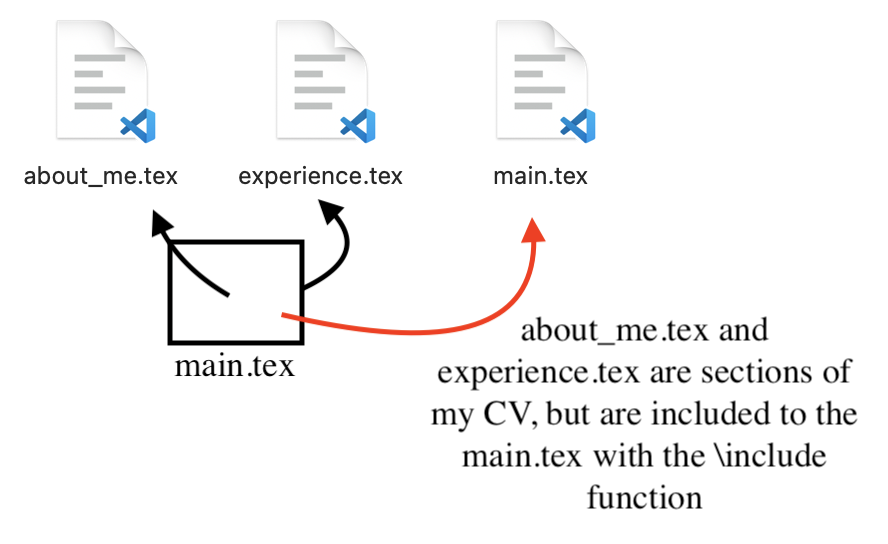
\includegraphics[scale=0.65]{latex.png}
\end{center}

%%%%%%%%%%%%%%%%%%%%%%%%%%%%%%%%%%%%%%%%%%%%%%%%%
\sectitle{HTML/CSS}

\paragraph{}
In the class, we learned how to use HTML (Hyper Text Markdown Language) and CSS (Cascade Style Sheet) to create simple websites. Like LaTeX, HTML is more like a markdown language than a programming language. It can be used just like LaTeX in different situations. I created my portfolio website using CSS features such as Flexbox and Grid. It helped me to create a responsive design for my website. Also, I found it very useful to organize some similar items into one class in the HTML document. It allowed me to avoid the first mistake of computer scientists: repeating myself. CSS also allows using relative size units like "rem" or "em". It is highly useful when it comes to creating websites that will be viewed on different screens. Additionally, percentages can be used to define relative sizes, just like I did when I was selecting a size for "grid-template-columns". Personal fonts can also be used in CSS. But, it is crucial to make sure that the machine of the user has access to the font. It can be achieved by providing some kind of font that is represented on some online website, or the font files with the extension woff/woff2 can be included in the files of the website, so that, when the user opened the website, it would upload the fonts from a server/backend/host. I used this feature to include my favorite "Inter" font on my portfolio website.
\begin{center}
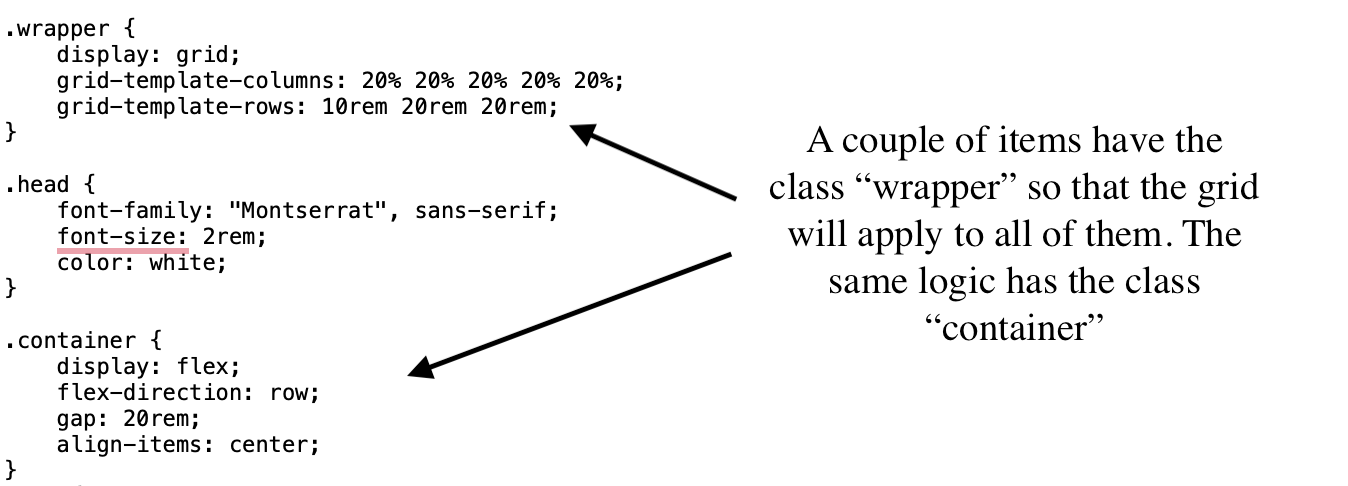
\includegraphics[scale=0.7]{web.png}
\end{center}

\sectitle{Jupyter Notebook}

\paragraph{}
In the class, Jupyter Notebook was introduced. Some beneficial features were presented. In my opinion, the most useful is the ability to include in the code whatever cell was previously executed (usually by referencing the number of the cell), the output of that cell, and interactivity with variables, i.e., if one value was given to a variable, it would spread across all future cells so that we could use it again without recreating the variable. We learned how to use some other features to analyze data. Since Jupyter Notebook is very interactive, it allowed us to write some documentation right inside the notebook using the markdown language. Also, Jupyter Notebook allows creating buttons and sliders to "play" with graphs. I used this feature in one of my graphs. 

\begin{center}
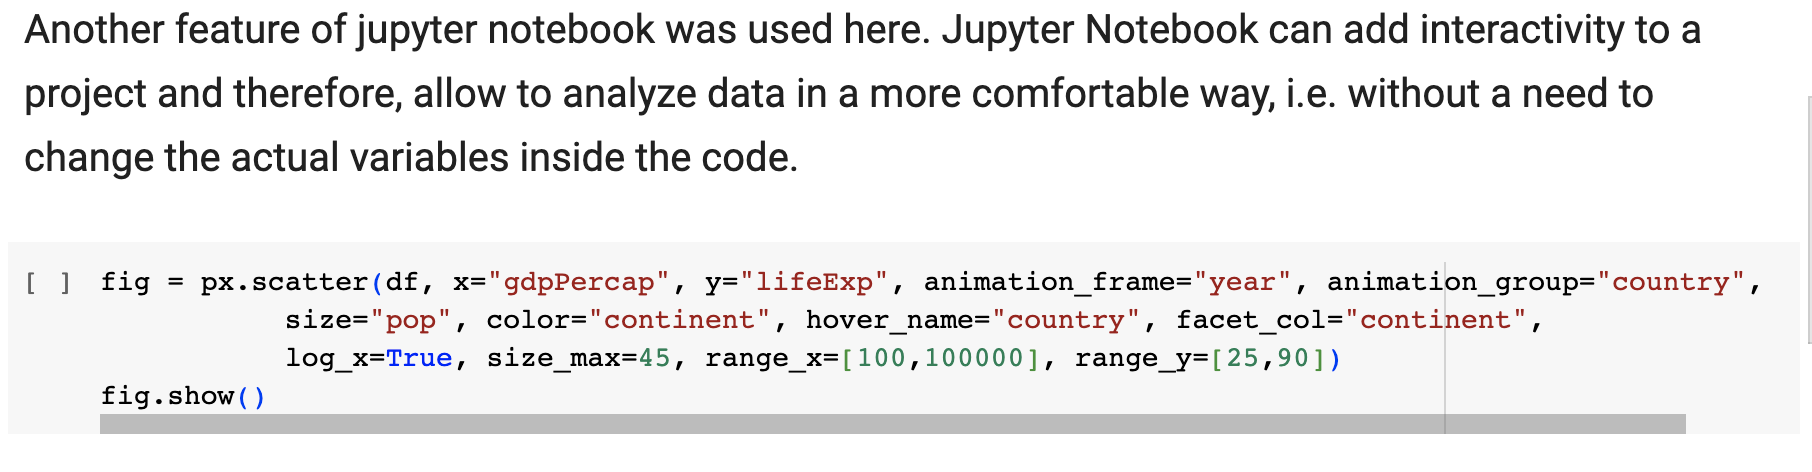
\includegraphics[scale=0.52]{jup1.png}
\end{center}

As seen in the picture, the project has the code and some documentation that was written using Markdown. There is a variable "df" that was defined at the start of the project, but I didn't have to redefine it in the current cell. 

\begin{center}
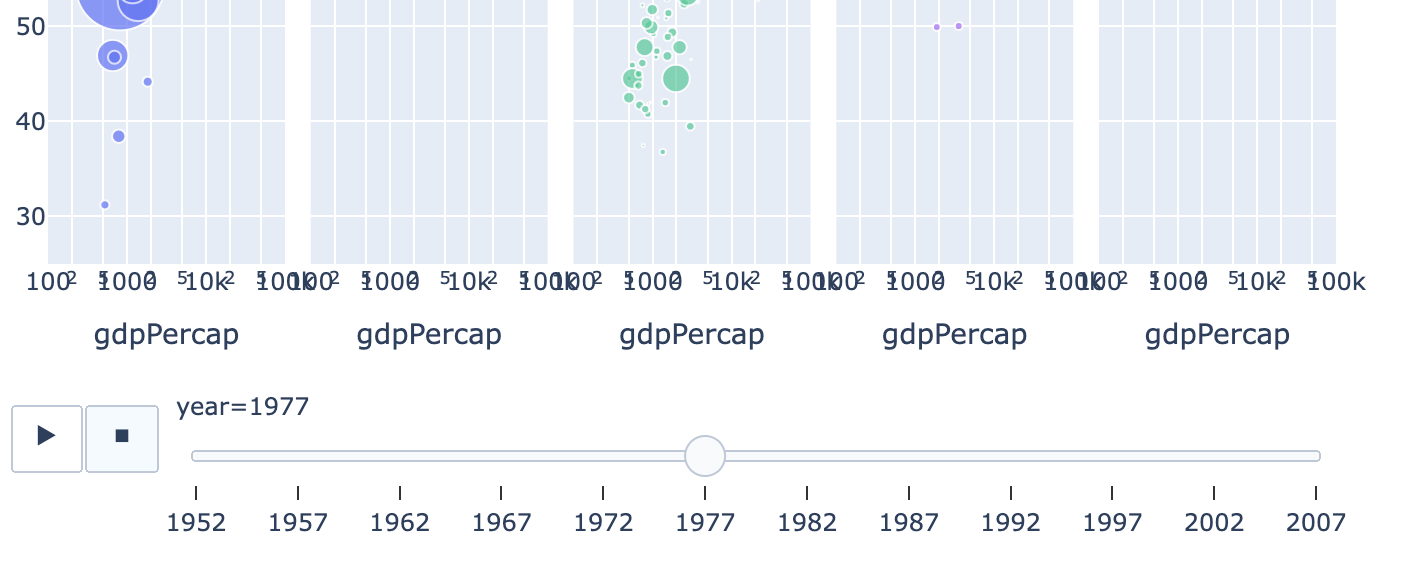
\includegraphics[scale=0.52]{jup2.png}
\end{center}

In this picture, some sliders can be seen. They allow us to change some variables in real-time so that we can see how the graph changes. 

\sectitle{Conclusion}
\paragraph{}
In conclusion, I would like to say that we have learned a lot of useful things that every successful computer scientist will use in the future. The class didn't end only on those mentioned. We learned how to use Linux shell and how to do version control by Git with a popular service called GitHub. The knowledge of how to use the Shell of a computer is extremely important for an IT specialist. Many things can't be done without Shell. All additional software, Python packages, and libraries can be downloaded only by using the terminal. It is worth mentioning that effective git version control also requires good Shell skills. Touch typing which we also learned in class now helps me a lot. My typing speed increased from 30 WPM to almost 60 WPM. I trained my touch typing on different websites such as typing academy and keybr. But, in my opinion, the most crucial part played was the fact that I didn't look at my keyboard while not particularly training in touch typing, i.e., since I had to write a lot to complete the university assignments I just practiced touch typing while I was writing the assignments. In my opinion, it was one of the most useful courses at the university so far!

\end{document}